\documentclass[10pt, conference, compsocconf]{IEEEtran}

%% Custom TeX

\usepackage{listings}
\usepackage{xcolor}
\usepackage{xspace}
\usepackage{graphicx}
\usepackage{caption}
\usepackage{subcaption}
\usepackage{rotating}
\usepackage{amssymb}
\usepackage{url}
\usepackage[splitrule]{footmisc}

%% for comments
\newcommand{\comment}[3][\color{red}]{{#1{[{#2}: {#3}]}}}
\newcommand{\code}[1]{\textsf{\small #1}}
\newcommand{\kris}[1]{\comment[\color{orange}]{km}{#1}}

\newcommand{\thickhline}{\noalign{\hrule height 1pt}}

%% End of custom TeX

\begin{document}
%
% --- Author Metadata here ---
% --- End of Author Metadata ---

\title{Using Big Data for Music Synthesis}

%%\numberofauthors{3}
\author{
\IEEEauthorblockN{Christopher Imbriano, Amanda Strickler, Kristopher Micinski
\IEEEauthorblockA{Computer Science Department, University of Maryland,
  College Park, MD 20742, USA\\
  \{micinski, pdphelp, jfoster\}@cs.umd.edu}
}

\maketitle

\begin{abstract}
\end{abstract}

\section{Introduction}
\label{sec:introduction}

The big data revolution has revolutionized the way we think about,
design, and implement algorithms at scale.  

We present a system to synthesize music using large amounts of data.
The input is a large corpus of images, which is subsequently processed
by our system, and the result is a musical score.

We study the music we 

\section{Overview}
\label{sec:overview}

The core idea in converting image data to music is to view the
information in an image (color, size, opacity, etc..) as a mapping to
notes and durations with which those notes are sustained.  In our
system we chose MIDI as the output format.  Our system can then be
modeled as a function \kris{transducer?} from image data to MIDI
output.  Note that the choice of MIDI limits the expressivity of our
music.  Going to other formats (e.g., MP3, OOG, etc..) could provide a
larger range of primitives with which to construct music, but does not
enjoy the simplicity that MIDI provides.

Our system is modeled as a function from ordered sets of images to a
MIDI file.  In our view, a MIDI file consists of note, duration pairs.


%% \[
%%     f : image^{\ast} \to (
%% \]

\paragraph{The HSB format}

To convert image data to musical notes, we need to establish a
bijection between the data in the image and the range of music in the
song.  The way we do this is inspired by viewing colors in images as
HSV values.  In HSV, each color has three components: a hue, a
saturation, and a value.  These components are visualized (as shown in
Figure~\ref{fig:hsv}) using a wheel.  The components represent:

\begin{describe}
\item[Hue] The actual ``color'' that would be described.  At full
  saturation and value, the hue determines the color seen.  This is
  visualized as going around a wheel of colors.

\item[Saturation] The degree to which the color is saturated from
  white.  Zero saturation is a blank (white) surface, while increasing
  values show more permeance of color.

\item[Value] The amount of light in the color.  Colors with low values
  are dark, and those with higher values are brighter.  This is
  visualized by going up the cylinder.
\end{describe}

\kris{Here I'm going to draw a diagram which shows two points on the
  HSV wheel and a musical clef, illustrating the position.}

\begin{figure}
  \centering
  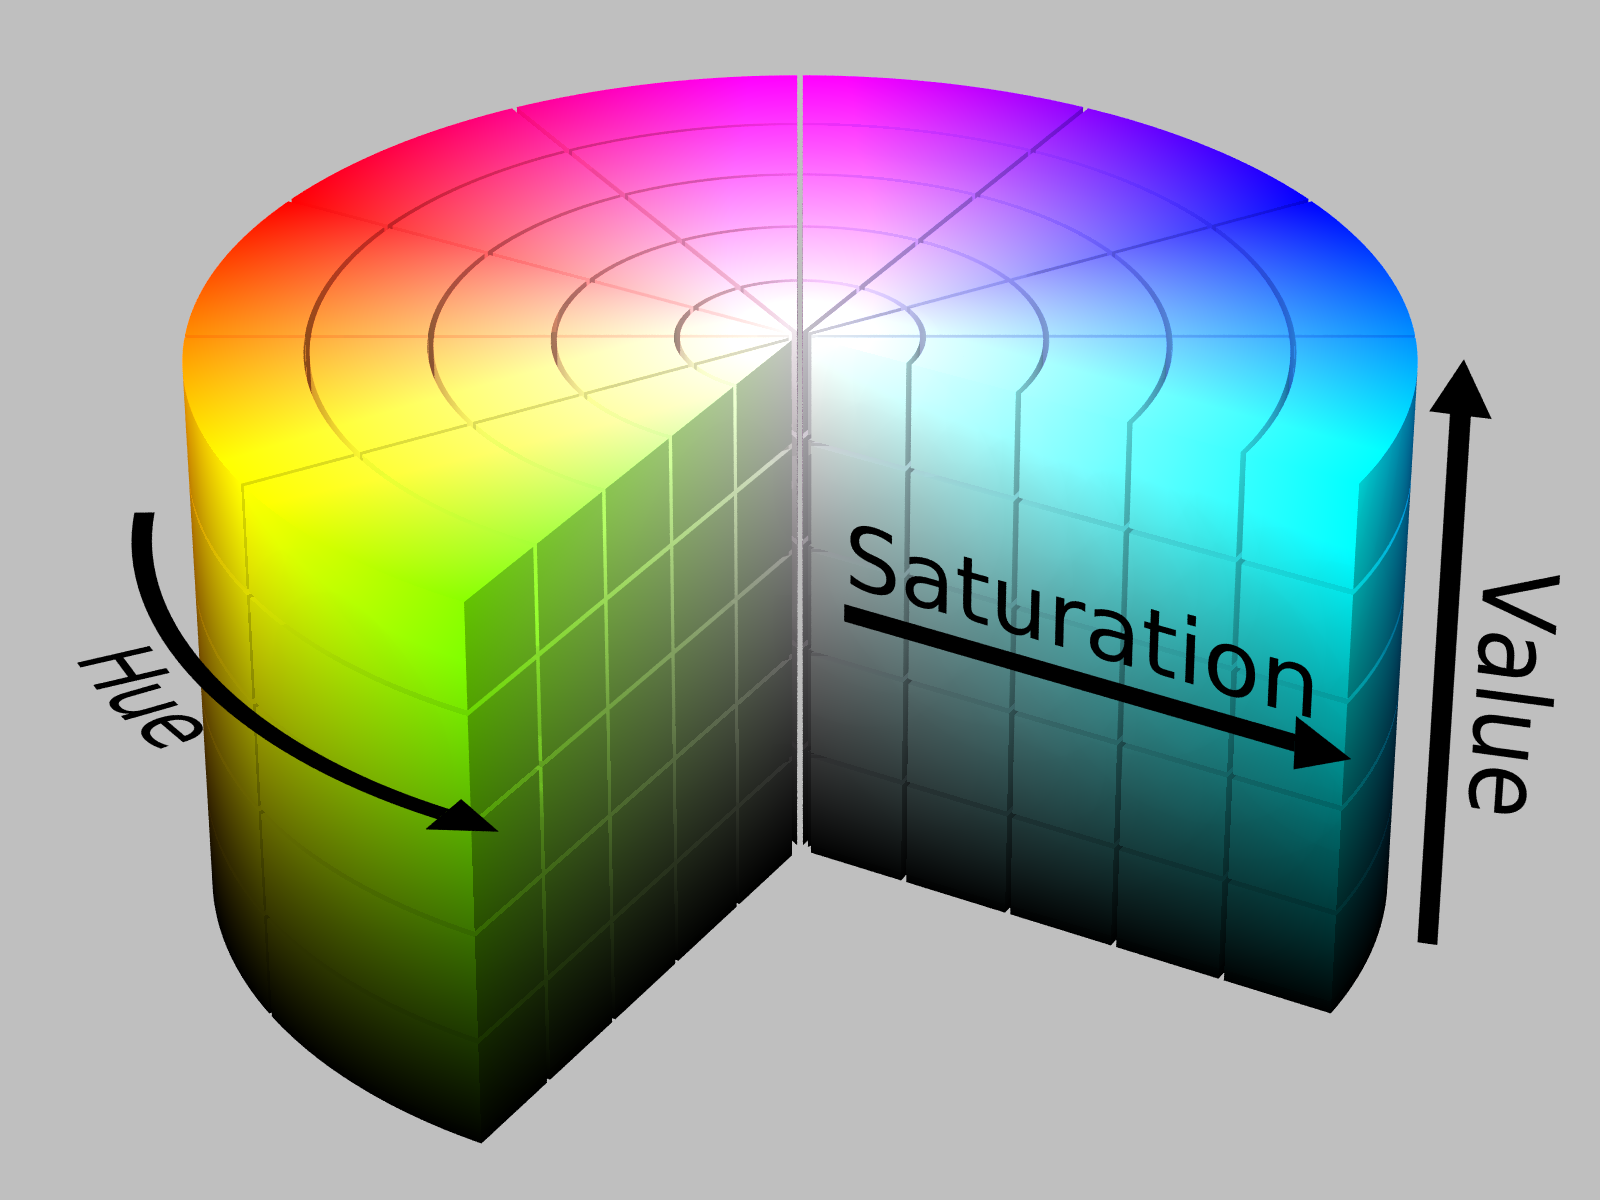
\includegraphics{hsv}
  \caption{The HSV color cylinder}
  \label{fig:hsv}
\end{figure}

\paragraph{Generating music}

To generate music, we take each image in our corpus and view it as a
single step in time.  Musical scores are made by streaming large
amounts of images.  (In fact, one possible idea is to use image data
from subsequent frames in movies to get streams of related images.)
Because our music would be relatively uninteresting if it had only one
``player'', we also include several \emph{regions} in the generated
music.  Each region is a distinct musical voice that can play
different notes and is mixed together with the rest of the music.  To
state this formally, each image is mapped to a set of regions and
notes:

\[
    f : A_{i,j} \to note^n
\]

where $i$ and $j$ are the dimensions of the image, and $n$ is the
number of distinct regions of the image.  The obvious idea is to
divide the image into $n$ distinct quadrants of equal size and project
the colors in that region to notes.  One problem is that we often deal
with relatively large images: if we have a smaller set of quadrants
how do we take this to a HSV value?  We solve this problem by taking
thumbnails of images, essentially doing a projection from $A_{i,j}$
down to $A_{n^{.5},n^{.5}}$.  This also tacitly stipulates that we
start out with square images (otherwise we lose some of the image data
in the projection): we handle this step as a first preprocessing
phase.

\section{Implementation}

\begin{figure}
  \centering
  \caption{High level view of the pipeline used for the project}
  \label{fig:project-pipeline}
\end{figure}

Our implementation consists of three MapReduce phases, tied together
with helper scripts.  The high level pipeline is shown in
Figure~\ref{fig:project-pipeline}.


\paragraph{Conversion to intermediate representation}
\label{sec:conversion}

Image data comes in a variety of different formats: JPEG, GIF, PNG,
etc..  Dealing with the plethora of formats presents a problem for our
translation because there are many artifacts of the formats
(annotations, geotagging, compression, etc..) which are unnecessary
for our implementation.  To keep the core abstraction of images as
arrays of bytes (the abstraction described in
Section~\ref{sec:overview}) the first stage of our Hadoop
implementation\footnote{\code{src/main/phase1}} converts the surface
image representation to the sequence file format used in subsequent
processing.  Although it may appear inefficient to hold an
uncompressed image in memory, this is actually ideal for Hadoop:
because computing cycles (incurred through recompressing and sending
the images) are the cost, compared with network traffic \kris{does
  this make sense???}.  

The conversion in our prototype uses the java \code{ImageBuffer} class
to do image input and conversion.  This class holds requires a large
amount of memory to represent image objects, however this is fine
because we hold only a small number of images in memory at any one
time (using statics) when mapping over our input corpus.

\paragraph{Translating to note, region pairs}

After taking the image data to an intermediate format, we must map the
image data to a set of note / region pairs for use in the MIDI.  To do
this, we do projection 

\section{Results}

\subsection{Sample datasets}

To test the system, we use a variety of different sets of images.
These images were obtained from
Flickr\footnote{\url{http://www.flickr.com/}}, using a public API and
a Python script \cite{flickerpy} \kris{Did we actually use this?  Did
  Amanda write the code?}  


\section{Related work}

Many domain specific programming languages exist for music synthesis
[\cite{haskore},\cite{lilypad}].  Many of these languages synthesize
music in the small ().  By contrast, our approach focuses on using
large amounts of data to create music...

\section{Conclusion}

\bibliographystyle{IEEEtran}
\bibliography{paper}

\end{document}
